\subsection{Address Translation}
\label{sec:paging}

System software relies on the CPU's address translation mechanism for
implementing isolation among less privileged pieces of software (applications
or operating systems). Virtually all secure architecture designs bring changes
to address translation. We summarize the Intel architecture's address
translation features that are most relevant when establishing a system's
security properties, and refer the reader to \cite{jacob1998virtual} for a more
general presentation of address translation concepts and its other uses.

From a systems perspective, address translation is a layer of indirection
between the \textit{virtual addresses}, which are used by a program's memory
load and store instructions, and the \textit{physical addresses}, which
reference the physical address space (\S~\ref{sec:address_spaces}). The mapping
between virtual and physical addresses is defined by \textit{page tables},
which are set up by system software.

\begin{figure}[hbt]
  \centering
  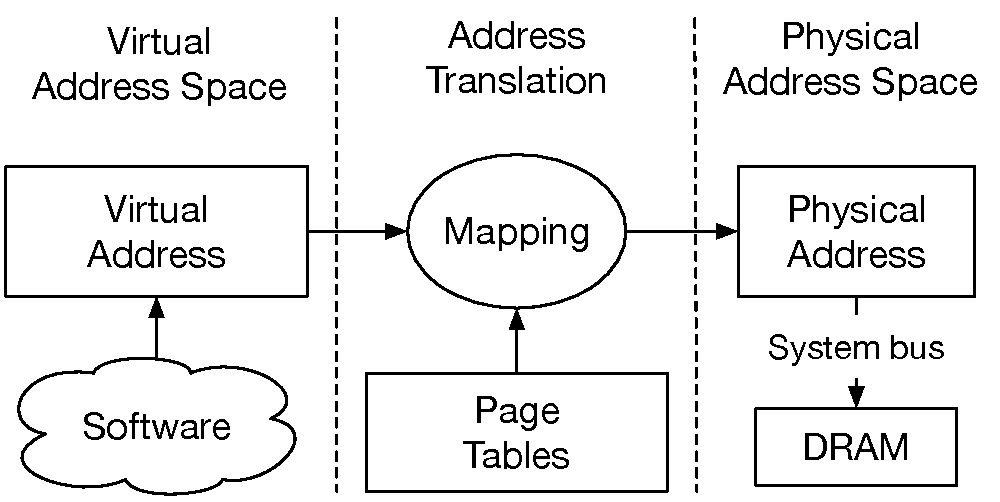
\includegraphics[width=75mm]{figures/address_translation.pdf}
  \caption{
    Virtual addresses used by software are translated into physical memory
    addresses using a mapping defined by the page tables.
  }
  \label{fig:address_translation}
\end{figure}

This mechanism lets the operating system multiplex DRAM among multiple
application processes, isolate the processes from each other, and prevent
application code from accessing memory-mapped devices directly. The latter two
protection measures prevent an application's bugs from impacting other
applications or the OS kernel itself. Hypervisors also use address translation,
to divide the DRAM among operating systems that run concurrently, and to
virtualize memory-mapped devices.

% Canonical Addressing: SDM vol1 S 3.3.7.1
% IA-32e Paging: SDM S 4.5

The address translation mode used by 64-bit operating systems, called
IA-32e by Intel's documentation, maps 48-bit \textit{virtual addresses} to
\textit{physical addresses} of at most 52 bits\footnote{The size of a
physical address is CPU-dependent, and is 40 bits for recent desktop CPUs and
44 bits for recent high-end server CPUs.}. Figure~\ref{fig:os_paging}
illustrates the process used to map a virtual address to a physical address.

\begin{figure}[hbtp]
  \centering
  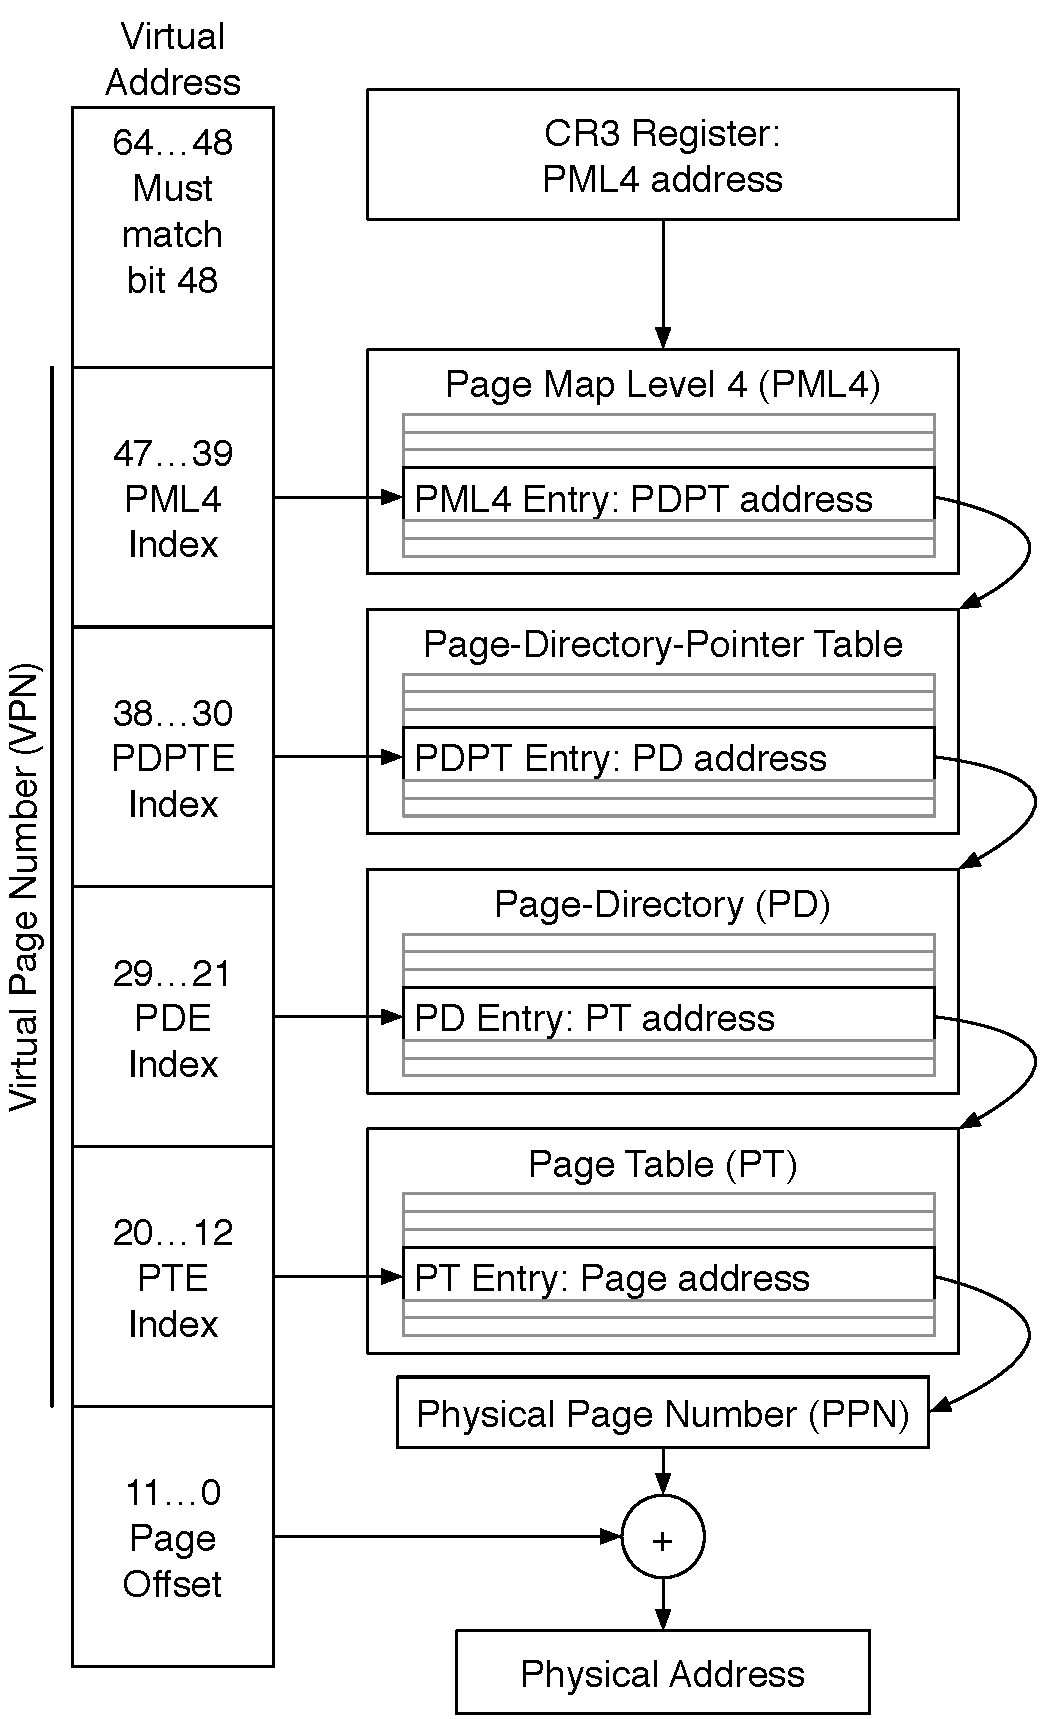
\includegraphics[width=85mm]{figures/os_paging.pdf}
  \caption{
    IA-32e address translation takes in a 48-bit virtual address and outputs
    a 52-bit physical address.
  }
  \label{fig:os_paging}
\end{figure}

The bottom 12 bits of a virtual address are not changed by the translation. The
top 36 bits are grouped into four 9-bit indexes, which are used to index into
the page tables. Despite its name, the page tables data structure closely
resembles a full 512-ary search tree where nodes have fixed keys. Each
node is represented in DRAM as an array of 512 8-byte entries that contain the
physical addresses of the next-level children as well as some flags. The
physical address of the root node is stored in the CR3 register. The arrays in
the last-level nodes contain the physical addresses that are the result of the
address translation.

% VMX Support for Address Translation: SDM S 4.11

Computers that take advantage of hardware virtualization use a hypervisor to
run multiple operating systems at the same time. This creates some tension,
because each operating system was written under the assumption that it owns the
entire computer's DRAM. The tension is solved by a second layer of address
translation, illustrated in Figure~\ref{fig:vmx_address_translation}.

\begin{figure}[hbt]
  \centering
  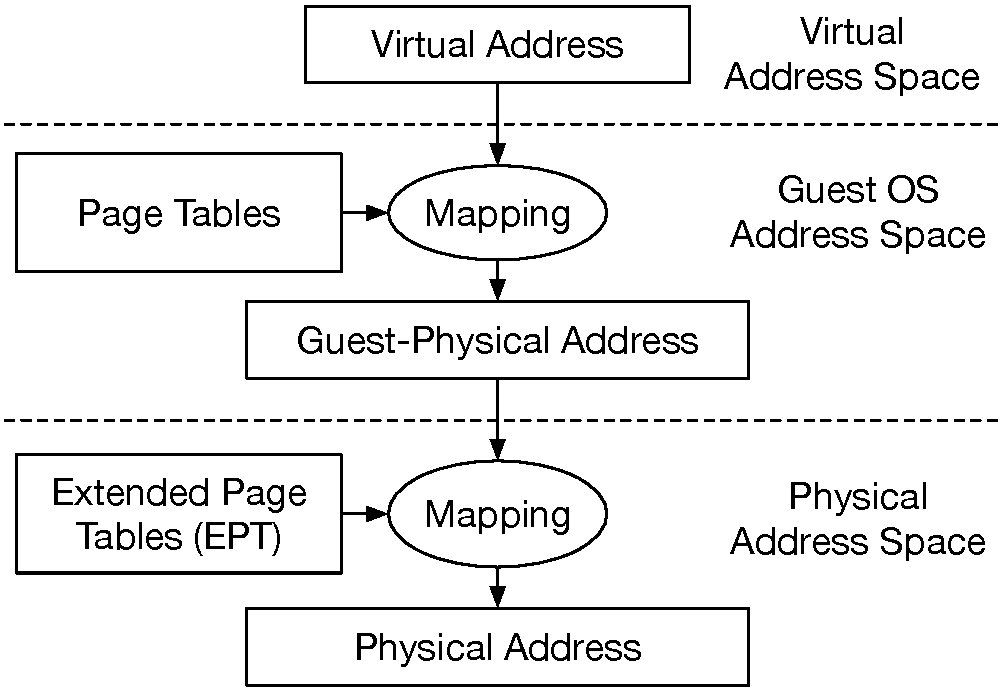
\includegraphics[width=70mm]{figures/vmx_address_translation.pdf}
  \caption{
    Virtual addresses used by software are translated into physical memory
    addresses using a mapping defined by the page tables.
  }
  \label{fig:vmx_address_translation}
\end{figure}


When a hypervisor is active, the page tables set up by an operating system map
between virtual addresses and \textit{guest-physical addresses} in a
\textit{guest-physical address space}. The hypervisor multiplexes the
computer's DRAM between the operating systems' guest-physical address spaces
via the second layer of address translations, which uses \textit{extended page
tables}~(EPT) to map guest-physical addresses to physical addresses.

The EPT uses the same data structure as the page tables, so the process of
translating guest-physical addresses to physical addresses follows the same
steps as IA-32e address translation. The main difference is that the physical
address of the data structure's root node is stored in the extended page table
pointer~(EPTP) field in the \textit{Virtual Machine Control Structure}~(VMCS)
for the guest OS. Figure~\ref{fig:vmx_paging} illustrates the address
translation process in the presence of hardware virtualization.

\begin{figure}[hbt]
  \centering
  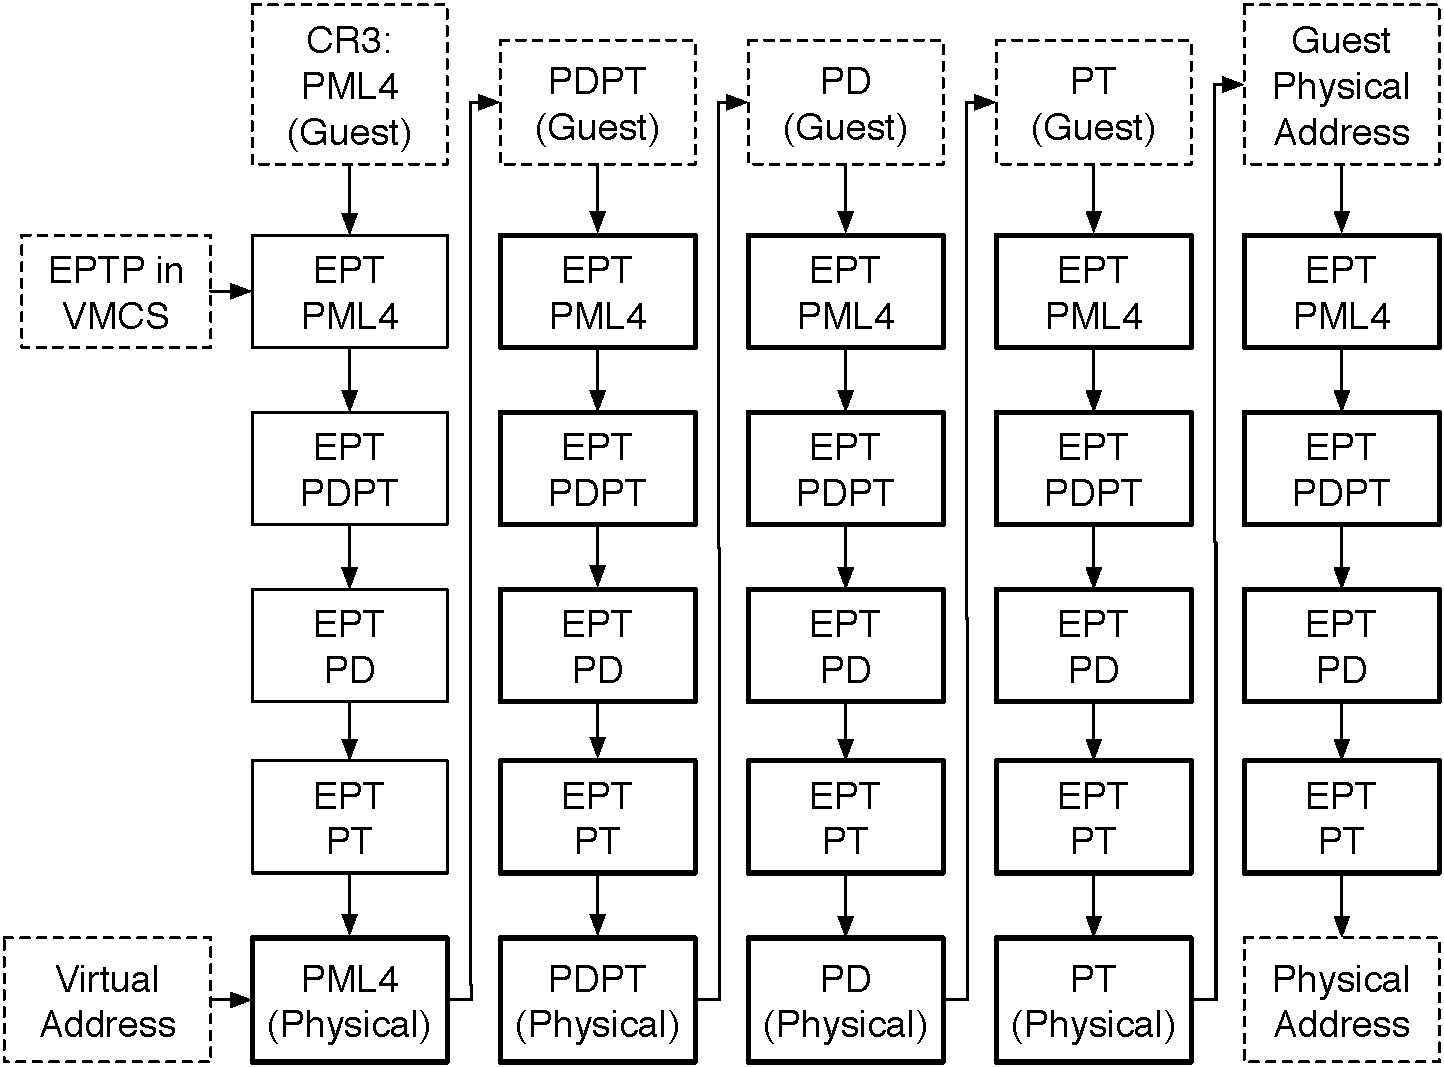
\includegraphics[width=85mm]{figures/vmx_paging.pdf}
  \caption{
    Address translation when hardware virtualization is enabled. The
    kernel-managed page tables contain guest-physical addresses, so each level
    in the kernel's page table requires a full walk of the hypervisor's
    extended page table~(EPT).  A translation requires up to 20 memory accesses
    (the bold boxes), assuming the physical address of the kernel's PML4 is
    cached.
  }
  \label{fig:vmx_paging}
\end{figure}

Each entry in the page tables has some Boolean flags, in addition to the
pointer to the next level. The following flags are particularly interesting for
our goals. The \textit{present}~(P) flag is set to 0 to indicate unused parts
of the address space, which do not have physical memory associated with them,
or pages that have been evicted from RAM to a cheaper and slower storage
medium.  The \textit{accessed}~(A) flag is set to 1 by the CPU whenever the
address translation machinery reads a page table entry, and the
\textit{dirty}~(D) flag is set to 1 by the CPU when an entry is accessed by a
memory write operation. The A and D flags give the hypervisor and kernel
insight into application memory access patterns, providing the input for the
algorithms that select which pages get to be evicted from RAM.

% Page-Level Protection: SDM S 5.11, S 5.11.{1,2,3,4}

Page table entries have flags that provide access control, in addition to the
flags supporting page swapping. The interesting flags are the
\textit{writable}~(W) flag, which can be set to 0 to prohibit\footnote{Writes
to non-writable pages result in \#GP exceptions (\S~\ref{sec:faults}).} memory
writes to a page, the \textit{disable execution}~(XD) flag, which can be set to
1 to prevent instruction fetches from a page, and the \textit{supervisor}~(S)
flag, which can be set to 1 to prohibit accesses from application software
running at ring 3.
